\documentclass[12pt]{amsart}
\usepackage{preamble}
\DeclareMathOperator{\stab}{\mathrm{stab}}

\begin{document}
\begin{center}
    \textsc{Math 601. HW 3\\ Ian Jorquera}
\end{center}
\vspace{1em}
\begin{itemize}
    % 8 points completed
    \item[(1)] % 5 points
    \begin{itemize}
        \item[(a)] % 1 point
        The following is the diagram representing $V^3$
        \begin{center}
            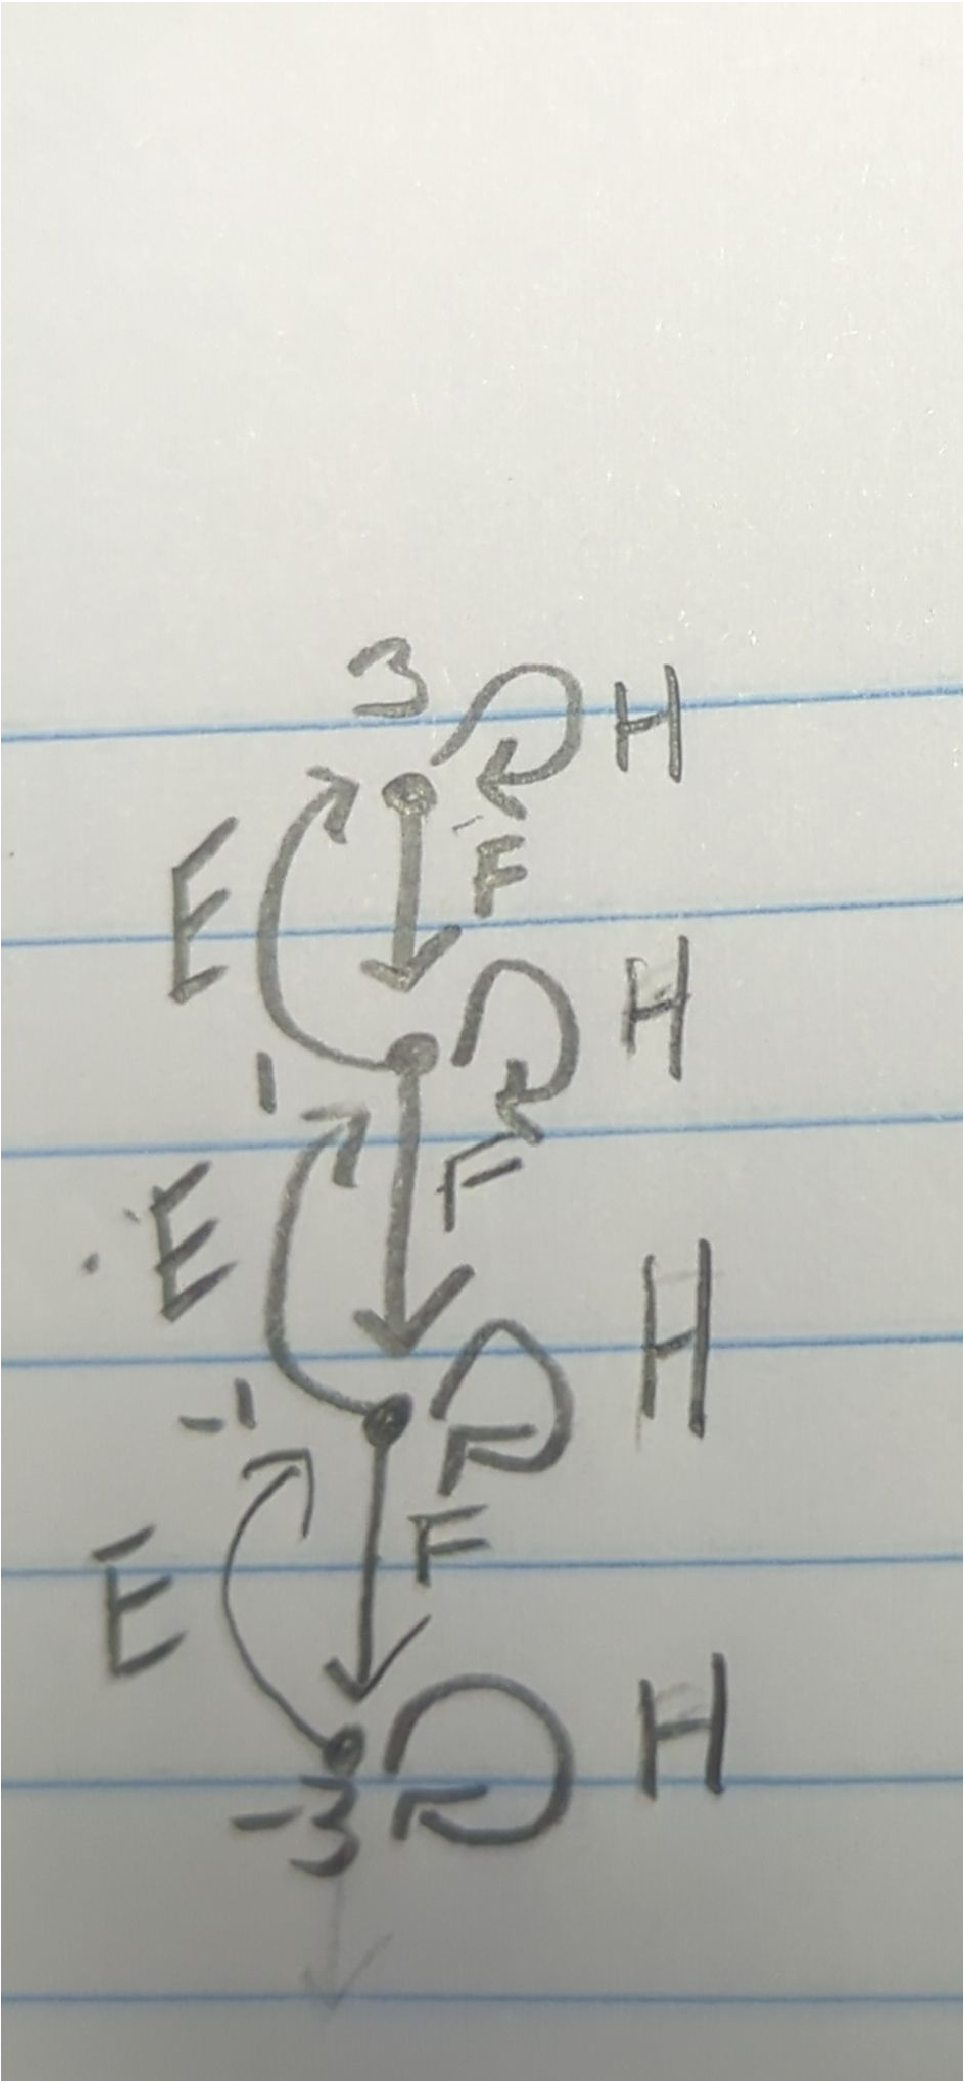
\includegraphics[width=1in]{hw3-1a.pdf}
        \end{center}
         
        \item[(b)] % 3 points
        Consider the representation $\rho:\mathfrak{sl}_2(\C)\ra\mathfrak{gl}_2(\C)=M_{4\times 4}(\C)$ 
        where we will fix the basis $\{v_3,v_1,v_{-1},v_{-3}\}$ In which case we know that we must map to matrices of the form
        \[F\mapsto\begin{bmatrix}
            0&0&0&0\\
            a&0&0&0\\
            0&b&0&0\\
            0&0&c&0
        \end{bmatrix}\]
        \[E\mapsto\begin{bmatrix}
            0&d&0&0\\
            0&0&e&0\\
            0&0&0&f\\
            0&0&0&0
        \end{bmatrix}\]
        \[H\mapsto\begin{bmatrix}
            3&0&0&0\\
            0&1&0&0\\
            0&0&-1&0\\
            0&0&0&-3
        \end{bmatrix}\]
        Furthermore we can use the first requirement of part $c$ that $[\rho(E),\rho(F)]=\rho(H)$ to find that $a=f=3$, $c=d=1$ and $b=e=2$ is a solution, giving
        \[F\mapsto\begin{bmatrix}
            0&0&0&0\\
            3&0&0&0\\
            0&2&0&0\\
            0&0&1&0
        \end{bmatrix}\]
        \[E\mapsto\begin{bmatrix}
            0&1&0&0\\
            0&0&2&0\\
            0&0&0&3\\
            0&0&0&0
        \end{bmatrix}\]
        \[H\mapsto\begin{bmatrix}
            3&0&0&0\\
            0&1&0&0\\
            0&0&-1&0\\
            0&0&0&-3
        \end{bmatrix}\]
        
        \item[(c)] % 1 point
         We can then check this in fact works as a representation with matlab 
        \begin{center}
            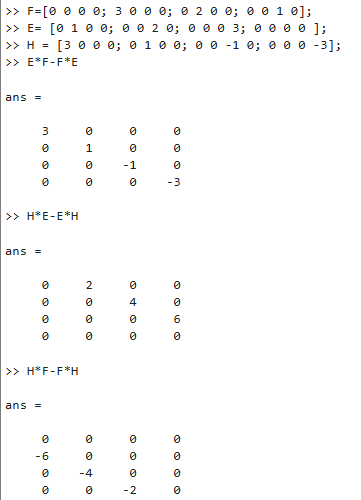
\includegraphics[width=3in]{hw3-1c.png}
        \end{center}
            
    \end{itemize}
    \item[(3)] % 3 points 
    First notice that the formal character of $V^2$ is $\rchi_{V^2}(q)=q^2+1+q^{-2}$
    And 
    \begin{align*}
        \rchi_{(V^2)^{\otimes 3}}(q)&=(\rchi_{V^2}(q))^3\\
        &=(q^2+1+q^{-2})^3\\
        &=q^6+3q^4+6q^2+7+6q^{-2}+3q^{-4}+q^{-6}\\
        &=(q^6+q^4+q^2+1+q^{-2}+q^{-4}+q^{-6})+2(q^4+q^2+1+q^{-2}+q^{-4})+3(q^2+1+q^{-2})+1\\
        &=\rchi_{V^6}(q)+\rchi_{V^4}(q)+\rchi_{V^4}(q)+\rchi_{V^2}(q)+\rchi_{V^2}(q)+\rchi_{V^2}(q)+\rchi_{V^0}(q)
    \end{align*}

    Meaning $(V^2)^{\otimes 3}=V^6\oplus V^4\oplus V^4\oplus V^2\oplus V^2\oplus V^2\oplus V^0$
\end{itemize}

\end{document}

